\section{A little bit of math}

\begin{frame}{Composition of functions} 
	\begin{columns}
		\begin{column}{.5\textwidth} 
			\begin{align}
				f(x)=& ax+b \\
				g(x)=&  \frac{1}{e^{-x}+1} \\
				g(f(x)) =& \frac{1}{e^{-(ax+b)}+1}   
			\end{align}
		\end{column}
		\begin{column}{.5\textwidth}
			\begin{figure}
				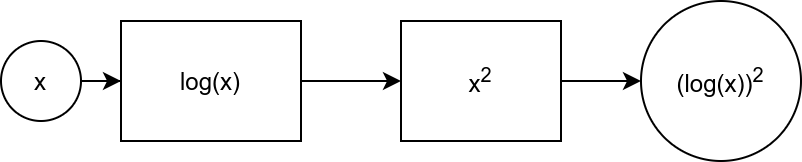
\includegraphics[width=.8\textwidth, center]{figures/function_composition}
				\caption*{Composite}
			\end{figure}
		\end{column}
	\end{columns}
\end{frame}

\begin{frame}{Derivatives}
	\begin{columns}
		\begin{column}{.5\textwidth}
			\begin{align}
				f(x)=&ax+b \\
				\frac{df(x)}{dx} =& a \\
				\sigma(z) =&\frac{1}{e^{-z}+1} \\
				\frac{d\sigma(z)}{dz} =& \sigma(z)(1-\sigma(z)) \\
				\frac{d\sigma(f(x))}{dx}=&?
			\end{align}
		\end{column}
		\begin{column}{.5\textwidth}
			\begin{figure}
				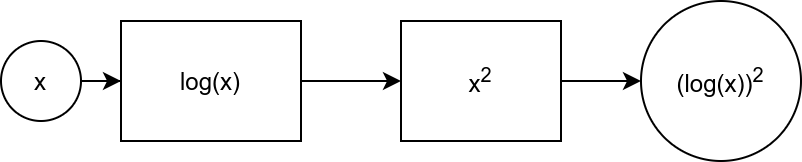
\includegraphics[width=.8\textwidth, center]{figures/function_composition}
				\caption*{Composite}
			\end{figure}
		\end{column}
	\end{columns}
\end{frame}

\begin{frame}{Derivatives}
	\begin{columns}
		\begin{column}{.5\textwidth}
			\begin{align}
				z=&ax+b \\
				\frac{dz}{dx} =& a \\
				\sigma(z) =&\frac{1}{e^{-z}+1} \\
				\frac{d\sigma}{dz} =& \sigma(z)(1-\sigma(z)) \\
				\frac{d\sigma}{dx}=&\frac{d\sigma}{dz} \frac{dz}{dx} 
			\end{align}
		\end{column}
		\begin{column}{.5\textwidth}
			\begin{figure}
				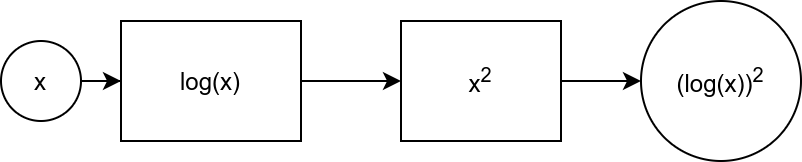
\includegraphics[width=.8\textwidth, center]{figures/function_composition}
				\caption*{Composite}
			\end{figure}
		\end{column}
	\end{columns}
\end{frame}


\begin{frame}{}
	\begin{columns}
		\begin{column}{.5\textwidth}
			\begin{align}
				z=&ax+b \\
				\frac{dz}{dx} =& a \\
				\sigma(z) =&\frac{1}{e^{-z}+1} \\
				\frac{d\sigma}{dz} =& \sigma(z)(1-\sigma(z)) \\
				\frac{d\sigma}{dx}=&\frac{d\sigma}{dz} \frac{dz}{dx}=\frac{dz}{dx} \frac{d\sigma}{dz}  
			\end{align}
		\end{column}
		\begin{column}{.5\textwidth}
			\begin{figure}
				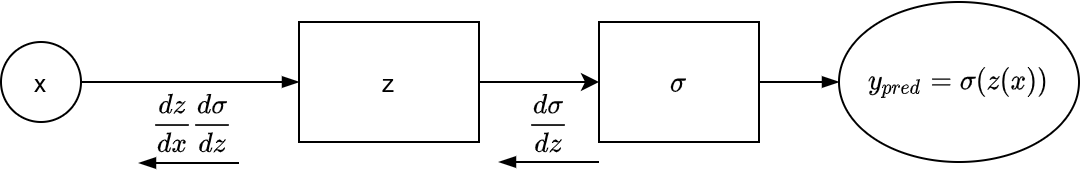
\includegraphics[width=.8\textwidth, center]{figures/function_composition_sigma}
				\caption*{Back propagation of gradients}
			\end{figure}
		\end{column}
	\end{columns}
\end{frame}